% =============================================================================
% COPYRIGHT AND DISCLAIMER
% =============================================================================
% This file is provided as a convenience template for competition participants.
% By using it, you accept full responsibility for compliance with all applicable
% copyright, licensing, and usage rules of the Association for Computing
% Machinery (ACM) and of any LaTeX packages you load (including, without
% limitation, the "acmart" document class and related ACM materials).
%
% Consult ACM's official publication, template, and copyright policies before
% using this setup for any purpose other than this competition. Do not assume
% that this template may be reused, redistributed, or submitted elsewhere
% without independently verifying ACM's current rules.
%
% Use of the "acmart" class, the "sigconf" option, or ACM-style formatting in
% this template does NOT mean that this report, this competition, its organizers,
% or any resulting PDF is sponsored, endorsed, affiliated with, or published by
% ACM. ACM trademarks and branding remain the property of ACM.
%
% Template packages live in preamble.tex.
% Citations live in main.bib. Edit this file with your paper content.
% =============================================================================

\documentclass[sigconf]{acmart}
% =============================================================================
% Template setup — participants normally do not edit this file.
% Author content belongs in main.tex; citations belong in main.bib.
% \documentclass lives in main.tex so Overleaf does not treat this file as root.
% =============================================================================

% --- Competition / non-ACM-submission friendly rights metadata -------------
\setcopyright{none}
\settopmatter{printacmref=false}
\acmConference[Kaggle Competition]{Filament Segmentation Challenge}{2026}{\href{https://www.kaggle.com/competitions/filament-segmentation-2026}{kaggle.com/competitions/filament-segmentation-2026}}
\acmBooktitle{Competition Report}
\acmDOI{}
\acmISBN{}

% --- Author guidance text --------------------------------------------------
% \guide{...} is gray italic while \guideStyletrue; omitted from the PDF if false.
% Flip the switch in main.tex after % =============================================================================
% Template setup — participants normally do not edit this file.
% Author content belongs in main.tex; citations belong in main.bib.
% \documentclass lives in main.tex so Overleaf does not treat this file as root.
% =============================================================================

% --- Competition / non-ACM-submission friendly rights metadata -------------
\setcopyright{none}
\settopmatter{printacmref=false}
\acmConference[Kaggle Competition]{Filament Segmentation Challenge}{2026}{\href{https://www.kaggle.com/competitions/filament-segmentation-2026}{kaggle.com/competitions/filament-segmentation-2026}}
\acmBooktitle{Competition Report}
\acmDOI{}
\acmISBN{}

% --- Author guidance text --------------------------------------------------
% \guide{...} is gray italic while \guideStyletrue; omitted from the PDF if false.
% Flip the switch in main.tex after % =============================================================================
% Template setup — participants normally do not edit this file.
% Author content belongs in main.tex; citations belong in main.bib.
% \documentclass lives in main.tex so Overleaf does not treat this file as root.
% =============================================================================

% --- Competition / non-ACM-submission friendly rights metadata -------------
\setcopyright{none}
\settopmatter{printacmref=false}
\acmConference[Kaggle Competition]{Filament Segmentation Challenge}{2026}{\href{https://www.kaggle.com/competitions/filament-segmentation-2026}{kaggle.com/competitions/filament-segmentation-2026}}
\acmBooktitle{Competition Report}
\acmDOI{}
\acmISBN{}

% --- Author guidance text --------------------------------------------------
% \guide{...} is gray italic while \guideStyletrue; omitted from the PDF if false.
% Flip the switch in main.tex after \input{preamble}.
%
% Do not use \guide{...} for \email{...}.
\usepackage{xcolor}
\newif\ifguideStyle
\guideStyletrue
\newcommand{\guide}[1]{%
  \ifguideStyle
    {\color{gray!65}\itshape #1}%
  \fi
}

% --- Math ------------------------------------------------------------------
% Do NOT load amssymb (or amsfonts): acmart already loads newtxmath, which
% defines the same symbols (e.g. \Bbbk) and causes a conflict on Overleaf.
% amsmath is already provided by acmart; mathtools extends it.
\usepackage{mathtools}

% --- Figures ---------------------------------------------------------------
% graphicx is already loaded by acmart
\usepackage{subcaption}

% --- Tables ----------------------------------------------------------------
% booktabs is already loaded by acmart
\usepackage{tabularx}
\usepackage{multirow}

% --- Bibliography style is set in main.tex (ACM-Reference-Format) ----------
.
%
% Do not use \guide{...} for \email{...}.
\usepackage{xcolor}
\newif\ifguideStyle
\guideStyletrue
\newcommand{\guide}[1]{%
  \ifguideStyle
    {\color{gray!65}\itshape #1}%
  \fi
}

% --- Math ------------------------------------------------------------------
% Do NOT load amssymb (or amsfonts): acmart already loads newtxmath, which
% defines the same symbols (e.g. \Bbbk) and causes a conflict on Overleaf.
% amsmath is already provided by acmart; mathtools extends it.
\usepackage{mathtools}

% --- Figures ---------------------------------------------------------------
% graphicx is already loaded by acmart
\usepackage{subcaption}

% --- Tables ----------------------------------------------------------------
% booktabs is already loaded by acmart
\usepackage{tabularx}
\usepackage{multirow}

% --- Bibliography style is set in main.tex (ACM-Reference-Format) ----------
.
%
% Do not use \guide{...} for \email{...}.
\usepackage{xcolor}
\newif\ifguideStyle
\guideStyletrue
\newcommand{\guide}[1]{%
  \ifguideStyle
    {\color{gray!65}\itshape #1}%
  \fi
}

% --- Math ------------------------------------------------------------------
% Do NOT load amssymb (or amsfonts): acmart already loads newtxmath, which
% defines the same symbols (e.g. \Bbbk) and causes a conflict on Overleaf.
% amsmath is already provided by acmart; mathtools extends it.
\usepackage{mathtools}

% --- Figures ---------------------------------------------------------------
% graphicx is already loaded by acmart
\usepackage{subcaption}

% --- Tables ----------------------------------------------------------------
% booktabs is already loaded by acmart
\usepackage{tabularx}
\usepackage{multirow}

% --- Bibliography style is set in main.tex (ACM-Reference-Format) ----------


% Guide styling: \guideStyletrue = show gray italic hints; \guideStylefalse = omit them
\guideStyletrue
% \guideStylefalse

\begin{document}

\title{EquiNexus: Grouped Validation and Family Voting for Solar Filament Segmentation}
\subtitle{A Solution to the Solar Filament Segmentation Challenge 2026} % DO NOT CHANGE


\author{\guide{Firstname Lastname}}
\affiliation{%
  \institution{\guide{Your Institution}}  % <- Optional (remove if you are not currently affiliated with any institute)
  \city{\guide{City}}
  \country{\guide{Country}}
}
\email{first.author@example.com}   % <- Replace with your own email

% \author{\guide{Second Author}}
% \affiliation{%
%   \institution{\guide{Your Institution}}  % <- Optional (remove if you are not currently affiliated with any institute)
%   \city{\guide{City}}
%   \country{\guide{Country}}
% }
% \email{second.author@example.com}  % <- Replace with your own email

\begin{abstract}
    This report describes EquiNexus's solution to the Solar Filament Segmentation Challenge~2026. We selected a label-free, three-family consensus of predictions from a U-Net/YOLO11s fusion, YOLO26x, and Mask R-CNN/refiner for the supplied test images. Among five completed uploads, Kaggle reference 58359982 received the highest public score, 0.40. The selected consensus has no EquiNexus OOF score. Its U-Net/YOLO11s component family reached PQ 0.459116 (95\% observation-bootstrap interval 0.4491--0.4692) at $c=0.25$ on 565 development observations and 922 annotator views. That grouped OOF result describes the component family, not the selected consensus. Public leaderboard scores are preliminary and are not independent estimates of private-set performance.
\end{abstract}

\maketitle





% ==================================== %
%              INTRODUCTION            %
% ==================================== %
\section{Introduction}
    This report goes over the details of our submitted solution to the Solar Filament Segmentation Challenge~2026 \cite{filament-segmentation-2026}. The challenge, launched on July~10,~2026, is organized by the Earth-Space AI Research (ESAIR) Lab\footnote{\href{https://www.esairlab.com/home}{www.esairlab.com/}}. This challenge utilizes the MAGFiLO dataset for evaluation of the segmentation algorithms \cite{ahmadzadeh2024dataset}. The supplied training partition contains 707 unique solar observations represented by 1,154 annotator views. We selected model and confidence settings using only competition-provided training annotations. The host's instance score compares predictions independently against each annotator's view, so our validation keeps every view from an observation in the same fold. We use the public leaderboard only to rank the final test submissions; it is a preliminary signal, not the basis for our validation claims.


% ==================================== %
%              METHODOLOGY             %
% ==================================== %
\section{Methodology}\label{sec:methodology}
    \subsection{Data split and model selection}
We froze the seed-42, year-stratified observation split before model comparison. The 20\% partition contains 142 observations; the remaining 565 observations form the development set. We assigned each original filename and all of its annotator views to one of five folds, with 113 observations per fold. The split manifest SHA-256 is \texttt{30cb2ec5...e48e}; the full digest and fold manifest are included in the repository. We did not stratify by observing site. Our five YOLO folds trained only on the development partition. The public U-Net model pool was trained on the competition training partition, which overlaps the reserved 142 observations. We therefore did not report a holdout score or treat that partition as an independent test of the combined system.

The public U-Net checkpoint collection contains five ResNet34 and five EfficientNetV2-S U-Nets. Its publisher reports training on the competition's training annotations, five image-grouped folds, and ImageNet-initialized encoders~\cite{afshar2026}. For OOF scoring, we used only the source-fold checkpoints that excluded each scored observation. For test inference, we averaged the ten-model ensemble. Each checkpoint predicts an image normalized by its mean and standard deviation inside a centered 950-pixel solar disk. Eight rotations/reflections are averaged. The published component rule keeps 8-connected regions above probability 0.35 when peak probability exceeds 0.99, mean probability is at least 0.85, and area is at least 200 pixels.

The second family is five YOLO11s-seg checkpoints trained on the 565-observation development partition. Each fold uses 452 observations for training and 113 for validation; the frozen 142-observation partition is excluded. We initialized from public COCO weights and used the Ultralytics implementation~\cite{ultralytics2026}, with image size 1,280, batch size two, and a maximum of 40 epochs with patience 12. At inference, each model processes the image under eight dihedral transforms; detections use NMS IoU 0.60 and at most 150 instances per transform. Duplicate augmented-view masks are suppressed at mask IoU 0.30. The detector confidence threshold is the only parameter varied in the final OOF sweep.

Table~\ref{tab:families} summarizes the roles of the two families. They make different errors: the U-Net supplies connected probability regions with a conservative component filter, while YOLO predicts separate instances with detector confidence. The family vote uses this difference as a support test. It is not a pixelwise average, and no extra model is fitted to the validation predictions.

\begin{table}[t]
\centering
\caption{Model families and inference roles.}
\label{tab:families}
\small
\begin{tabularx}{\columnwidth}{lXX}
\toprule
Family & Training or source & Inference output \\
\midrule
Public U-Net & Five ResNet34 and five EfficientNetV2-S checkpoints; ImageNet encoder initialization; published grouped training & Eight-view probability ensemble; component-filtered instances \\
YOLO11s-seg & Five folds; 452 training and 113 validation observations per fold; COCO initialization & Eight-view instance detections; confidence filter and mask-IoU deduplication \\
\bottomrule
\end{tabularx}
\end{table}

\subsection{Cross-family instance voting}
For each image, the U-Net and YOLO families propose candidate instance masks. A candidate is retained when an instance from the other family overlaps it at IoU strictly greater than 0.50. A mask with support can therefore appear once from each family; overlapping pixels are resolved in a fixed family-priority order, accepting a mask only if at least half of its area remains after clipping. If no mask receives cross-family support, we keep the stable highest-vote fallback, ordered by vote count, U-Net priority, detector confidence, and original index. This avoids empty outputs while retaining deterministic behavior.

The submitted test file extends this family vote with two independent prediction sources: HDJoJo YOLO26x and the I079 Mask R-CNN/refiner. A mask enters the consensus with support from at least two of the three families at IoU $>0.50$. When exactly two families support it, both must reach IoU $\geq0.60$. Overlap clipping retains at least half of a mask's pixels; an image with no qualifying consensus receives one deterministic highest-vote fallback. The builder reads only the three prediction CSVs and the supplied test filenames. It does not read test-image pixels or labels. The three-family output was not scored on EquiNexus's grouped OOF partition.

We assign unique per-image filament IDs after clipping and encode each 2048$\times$2048 mask as COCO run-length encoding (RLE). The final validator checks that every supplied test image appears, masks decode to the expected shape, IDs are unique, masks are nonempty, and masks within an image do not overlap. Empty images are represented by no instance rows. These checks are run on every candidate before submission and again on the selected package's reproduction output.

\begin{figure*}[t]
\centering
\setlength{\tabcolsep}{2pt}
\begin{tabular}{c c c c c c c c c c c}
\fbox{\parbox[c][0.72in][c]{0.118\textwidth}{\centering\scriptsize Official training\\707 observations\\1,154 views}} & $\longrightarrow$ &
\fbox{\parbox[c][0.72in][c]{0.118\textwidth}{\centering\scriptsize Grouped models\\5 YOLO11s folds\\10 public U-Nets}} & $\longrightarrow$ &
\fbox{\parbox[c][0.72in][c]{0.118\textwidth}{\centering\scriptsize Supplied test set\\180 H-$\alpha$ images\\no test labels}} & $\longrightarrow$ &
\fbox{\parbox[c][0.72in][c]{0.118\textwidth}{\centering\scriptsize Eight-view D4\\YOLO and U-Net\\mask ensembles}} & $\longrightarrow$ &
\fbox{\parbox[c][0.72in][c]{0.118\textwidth}{\centering\scriptsize Three-family vote\\IoU $>0.50$\\disjoint masks}} & $\longrightarrow$ &
\fbox{\parbox[c][0.72in][c]{0.118\textwidth}{\centering\scriptsize Instance IDs\\COCO RLE\\submission.csv}}
\end{tabular}
\caption{End-to-end pipeline. External initialization uses public ImageNet and COCO weights; task-specific training uses only competition-provided training annotations.}
\label{fig:pipeline}
\end{figure*}

% ==================================== %
%              EVALUATION              %
% ==================================== %
\section{Evaluation}\label{sec:evaluation}
    \subsection{Official grouped evaluation}
We ported the organizer's self-evaluation logic without changing its IoU threshold or matching rule~\cite{officialscorer2026}. A pair counts as a true positive only when IoU is strictly greater than 0.50; every qualifying pair counts, with no one-to-one assignment. Unmatched prediction and ground-truth instances count as false positives and false negatives. Each observation's prediction is evaluated against each annotator view. PQ is the sum of qualifying-pair IoUs divided by $TP+0.5FP+0.5FN$.

On the 565-observation, five-fold OOF partition, confidence $c=0.25$ produced PQ 0.459116 (TP 4,008; FP 1,502; FN 2,480; 922 annotator views). A 20,000-resample bootstrap over original observations gave a 95\% interval of 0.4491--0.4692. In a paired bootstrap, the family vote exceeded the public U-Net OOF baseline by 0.00556 (95\% interval 0.00261--0.00846; probability of improvement 0.99995). This paired comparison uses the same observation resamples; it is stronger evidence than comparing unrelated upstream scores. The interval conditions on the selected configuration and does not correct for searching nine confidence thresholds.

Table~\ref{tab:folds} shows the pooled score within each held-out fold. Each fold has 113 original observations; the number of annotator views varies because some observations have multiple expert annotations. Fold 1 is the strongest at 0.483, while the other four range from 0.451 to 0.454. This spread indicates that the pooled score averages over meaningful differences in observation difficulty and annotator-view count.

\begin{table}[t]
\centering
\caption{OOF scores by held-out observation fold at confidence 0.25.}
\label{tab:folds}
\small
\begin{tabular}{crrrr}
\toprule
Fold & Views & PQ & FP & FN \\
\midrule
0 & 188 & 0.451 & 334 & 486 \\
1 & 183 & 0.483 & 289 & 455 \\
2 & 185 & 0.454 & 291 & 535 \\
3 & 179 & 0.453 & 265 & 493 \\
4 & 187 & 0.454 & 323 & 511 \\
\bottomrule
\end{tabular}
\end{table}

The confidence search was performed once on cached cross-fitted predictions. Table~\ref{tab:sweep} reports the full grid so the choice of fresh uploads can be audited. Four distinct U-Net/YOLO11s test files were selected in descending frozen OOF PQ order after previously submitted hashes and a duplicate test output were excluded. A separate three-family test consensus provided a fifth, diverse candidate. The consensus has no EquiNexus OOF metric.

\begin{table}[t]
\centering
\caption{Frozen OOF confidence sweep.}
\label{tab:sweep}
\small
\begin{tabular}{rcl}
\toprule
Confidence & OOF PQ & Batch status \\
\midrule
0.21 & 0.457996 & -- \\
0.22 & 0.458361 & -- \\
0.23 & 0.458308 & -- \\
0.24 & 0.458726 & candidate 2 \\
0.25 & 0.459116 & candidate 1 \\
0.26 & 0.458816 & same test bytes as 0.25 \\
0.27 & 0.458678 & candidate 3 \\
0.28 & 0.458367 & candidate 4 \\
0.29 & 0.457936 & -- \\
\bottomrule
\end{tabular}
\end{table}

The four confidence variants describe one model family and share its OOF protocol; the three-family consensus is a test-only candidate with no EquiNexus OOF score. Public leaderboard scores are reported separately from validation evidence.

\begin{table}[t]
\centering
\caption{Nov.~14 upload batch. Public values are Kaggle leaderboard scores; OOF values use the official grouped scorer. The consensus has no EquiNexus OOF score.}
\label{tab:submissions}
\small
\begin{tabularx}{\columnwidth}{Xccc}
\toprule
Candidate & OOF PQ & Public PQ & Kaggle ref \\
\midrule
U-Net + YOLO11s, $c=0.25$ & 0.459116 & 0.39 & 58359833 \\
U-Net + YOLO11s, $c=0.24$ & 0.458726 & 0.39 & 58359863 \\
U-Net + YOLO11s, $c=0.27$ & 0.458678 & 0.39 & 58359890 \\
U-Net + YOLO11s, $c=0.28$ & 0.458367 & 0.39 & 58359925 \\
Three-family consensus & n/a & \textbf{0.40} & \textbf{58359982} \\
\bottomrule
\end{tabularx}
\end{table}

All five submissions completed by 7:06 PM Toronto time. We selected Kaggle reference \texttt{58359982}, the three-family consensus, because its public score of 0.40 exceeded the 0.39 score of each confidence variant. The OOF ranking did not determine this selection. This public score is a leaderboard result, not a final private-set measurement.

\subsection{Cross-site and temporal behavior}
At $c=0.25$, OOF PQ ranged from 0.441 at Mh to 0.472 at Th across the six observing sites. Table~\ref{tab:site} reports site-level counts using the same view-wise scorer. These values are descriptive: the validation folds were stratified by year, not site, and the later years have fewer annotator views. For temporal context, grouped scores were 0.461 for 2011--2013, 0.456 for 2014--2016, 0.467 for 2017--2019, and 0.453 for 2020--2022. The last two ranges contain only 146 and 61 views, respectively, so their point estimates are less stable.

\begin{table}[t]
\centering
\caption{OOF PQ by observing site. Each observation prediction is scored against each annotator view.}
\label{tab:site}
\small
\begin{tabular}{lrrr}
\toprule
Site & Views & PQ & TP / FP / FN \\
\midrule
Bh & 148 & 0.464 & 689 / 274 / 403 \\
Ch & 152 & 0.455 & 721 / 240 / 483 \\
Lh & 165 & 0.454 & 669 / 265 / 437 \\
Mh & 172 & 0.441 & 642 / 280 / 418 \\
Th & 143 & 0.472 & 689 / 232 / 402 \\
Uh & 142 & 0.470 & 598 / 211 / 337 \\
\bottomrule
\end{tabular}
\end{table}

\subsection{Instance and morphology diagnostics}
At any positive overlap (IoU $>0$), the evaluation contained 5,021 intersecting prediction--truth pairs, with mean pair IoU 0.614 and mean Dice 0.743. The stricter official match threshold yielded 4,008 true-positive pairs. At the diagnostic threshold, 154 ground-truth instances overlapped two or three predictions, while 103 predictions overlapped two or three ground-truth instances. These split and merge indicators help distinguish boundary disagreement from fragmentation; they do not replace the official PQ calculation.

The overlays in Figure~\ref{fig:overlays} show that the ensemble generally follows the dominant curved filament traces, while faint branches and narrow endpoints are more often omitted. Short isolated false positives remain around low-contrast structures. Because annotations from different experts do not always share identical boundaries or instance splits, we interpret these examples as both model error and annotation variation. We did not postprocess masks to enforce a solar-physics morphology prior, so apparent continuity is assessed visually rather than imposed by a hand-coded shape rule.

\subsection{Inference cost}
The ten-model U-Net replay took 1,293.8 seconds and reached 2.46 GiB peak allocation; five-fold YOLO inference took 4,149.7 seconds and reached 1.39 GiB. The complete local run, including deduplication, family voting, and RLE validation, took 5,569.7 seconds on an NVIDIA GeForce RTX 5070 Laptop GPU with 8 GB of VRAM. The run metadata records package versions, checkpoint hashes, component runtimes, and memory. These timings describe this laptop and are not directly comparable to Kaggle hardware. The inference notebook loads fixed weights and does not retrain the models.

\subsection{Qualitative behavior and limitations}
Figure~\ref{fig:overlays} shows three OOF examples. Green pixels are present only in the first annotator's ground-truth union, red pixels only in the prediction, and yellow pixels in both. The visual panels show one annotator view for readability; each reported PQ uses all views for the observation. The examples show agreement on the main filament traces alongside missed faint structures and short isolated false positives. Expert boundaries and instance splits vary, so some apparent errors also reflect annotation disagreement.

\begin{figure}[tb]
\centering
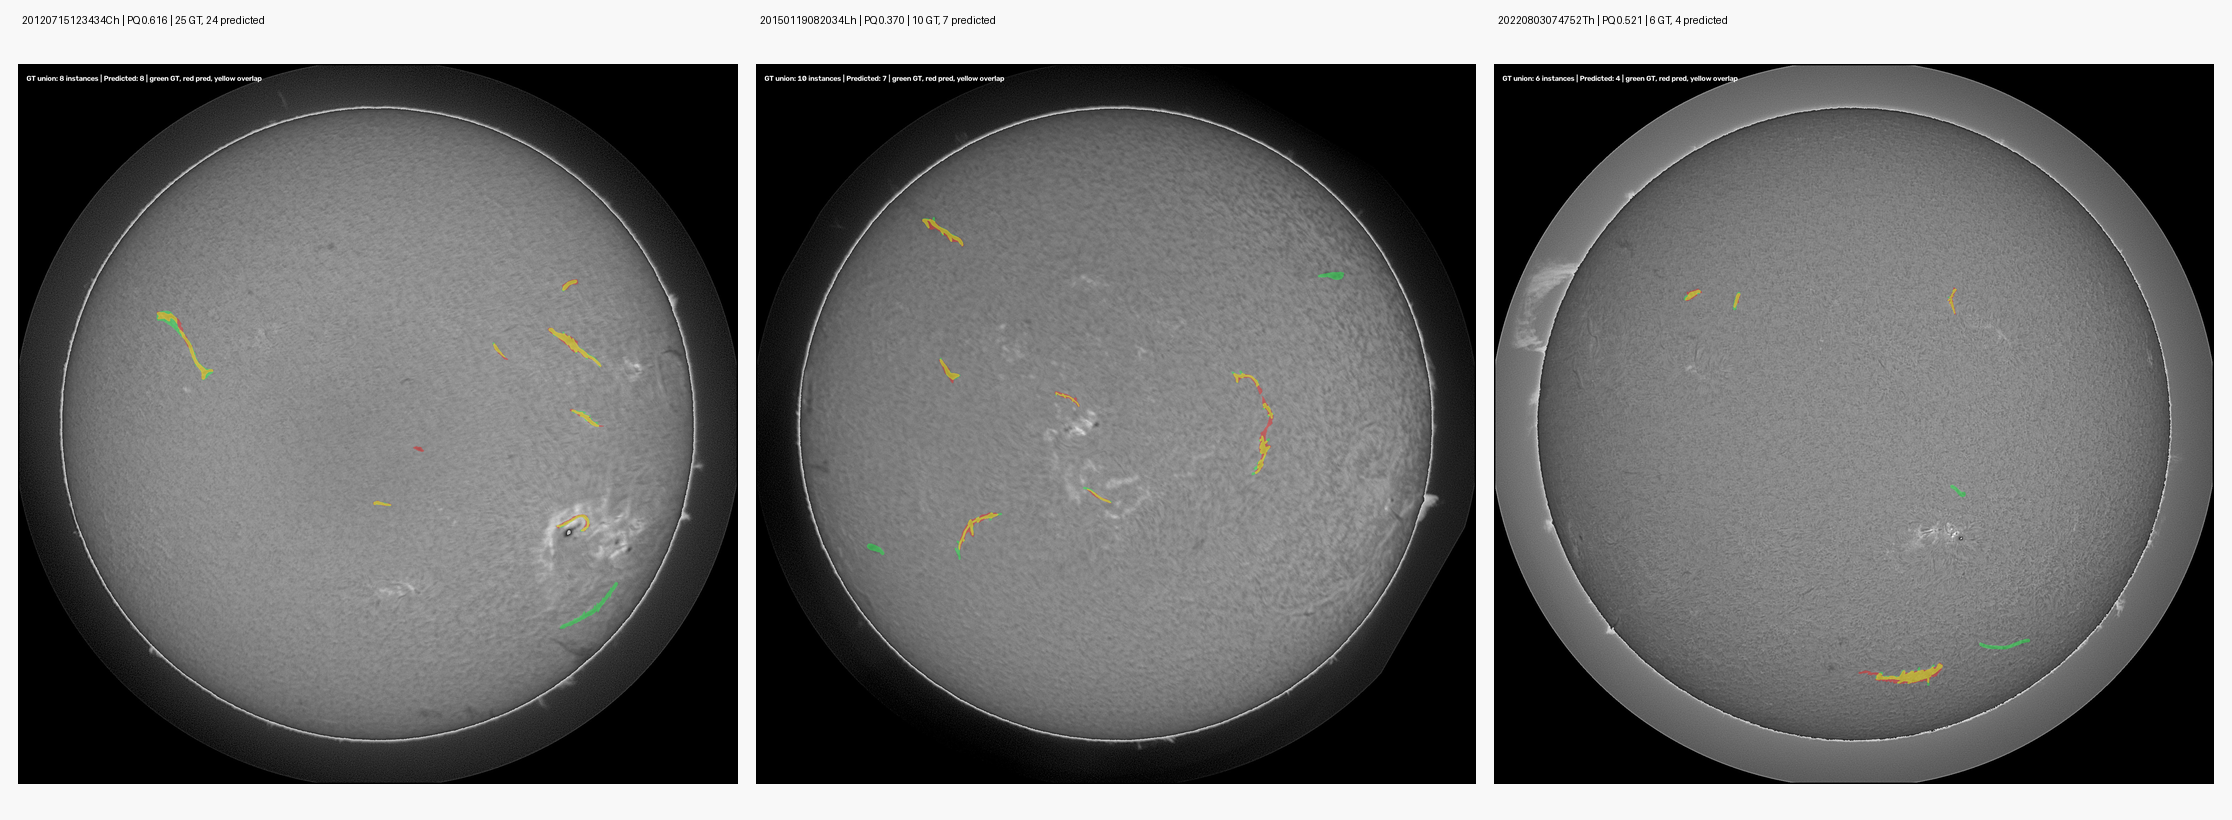
\includegraphics[width=\columnwidth]{figures/validation-oof-overlays.png}
\caption{First-annotator overlays from OOF observations. Green: ground-truth-only; red: prediction-only; yellow: overlap. The per-panel OOF PQ aggregates all annotator views for that original observation.}
\label{fig:overlays}
\end{figure}

The OOF score estimates performance on the 565-observation development subset. We did not evaluate the combined system on the reserved 142 observations: the public U-Net pool was trained on portions of that set, so it is not an independent holdout for this ensemble. For OOF predictions, each evaluated development observation uses the U-Net source fold that excluded it and the YOLO fold that held it out. For test inference, the U-Net pipeline averages all ten public checkpoints and the detector averages five development folds; this difference in training data and ensemble size is a train--test mismatch. Threshold search also makes the selected OOF point optimistic, even though the reserved partition was not used for threshold selection. Finally, the public leaderboard reflects only its evaluation partition and may rank candidates differently from the private score. We therefore report validation, upstream checkpoint claims, and leaderboard scores separately.

All task-specific training used competition-provided training annotations; test inference used only the supplied H-$\alpha$ test images. Public MAGFiLO labels for test observations were not accessed. The redistributed U-Net checkpoints retain the upstream CC BY-NC-SA 4.0 attribution and ShareAlike terms; the EquiNexus YOLO code and fine-tuned weights retain AGPL-3.0 notices. The HDJoJo YOLO26x and I079 detector/refiner retain their Apache-2.0 terms~\cite{afshar2026,ultralytics2026,hdjojo2026,i0792026}. Public ImageNet/COCO initialization is documented in the source manifests.



% ==================================== %
%            ACKNOWLEDGMENT            %
% ==================================== %
\section{Acknowledgment}\label{sec:acknowledgment}
    % Do not change
    The organization of the Filament Segmentation Challenge 2026 is partially supported by the U.S. National Science Foundation (NSF) under Grant No. 2209912 and 2433781, directorate for Computer and Information Science and Engineering (CSE), and Office of Advanced Cyberinfrastructure (OAC), and Grant No. 2511630, AST Division Of Astronomical Sciences and MPS Directorate for Mathematical and Physical Sciences.

    The Filament Segmentation Challenge 2026 is sponsored by the U.S. National Science Foundation (NSF) National Solar Observatory (NSO).

    This work utilizes GONG data obtained by the NSO Integrated Synoptic Program, managed by the National Solar Observatory, which is operated by the Association of Universities for Research in Astronomy (AURA), Inc. under a cooperative agreement with the National Science Foundation and with contribution from the National Oceanic and Atmospheric Administration. The GONG network of instruments is hosted by the Big Bear Solar Observatory, High Altitude Observatory, Learmonth Solar Observatory, Udaipur Solar Observatory, Instituto de Astrofísica de Canarias, and Cerro Tololo Interamerican Observatory.

\bibliographystyle{ACM-Reference-Format}
\bibliography{main}

\end{document}
